\documentclass[11pt,a4paper]{article}

\usepackage[T1]{fontenc}
\usepackage[utf8]{inputenc}
\usepackage[margin=2.5cm]{geometry}
\usepackage{amsmath,amssymb}
\usepackage{graphicx}
\usepackage{booktabs}
\usepackage{circuitikz}
\usepackage{listings}
\usepackage{xcolor}
\usepackage{hyperref}

\lstset{
  basicstyle=\ttfamily\footnotesize,
  keywordstyle=\bfseries,
  commentstyle=\color{gray},
  breaklines=true,
  frame=single,
  numbers=left,
  numberstyle=\tiny\color{gray},
  xleftmargin=2em
}

\newcommand{\ud}{\mathrm{d}}

\title{Active Clamping of High-Voltage IGBTs:\\
Theory, Design for a 6.5\,kV\,/\,1000\,A Module\\
and a Simscape TVS Model}
\author{Davide Bagnara}
\date{\today}

\begin{document}
\maketitle

\begin{abstract}
Active clamping is a gate-side overvoltage protection technique in which
the collector--emitter voltage of an IGBT is fed back to the gate through
a stack of transient voltage suppressor (TVS) diodes. When the collector
voltage exceeds the stack breakdown level, the device is forced back into
linear conduction and absorbs the inductive commutation energy while its
voltage is limited to the clamp level. This note reviews the operating
principle and its variants, develops a complete design procedure for the
6.5\,kV\,/\,1000\,A HiPak module 5SNA~1000G650300, including tolerance,
temperature and energy budgets, the adiabatic thermal capability of the
die and the coordination with an external MOV clamp, and documents \texttt{tvs\_clamp}, a Simscape component modelling
the TVS stack for time-domain verification together with the
\texttt{igbt\_dyn} switching model.
\end{abstract}

\tableofcontents

%=====================================================================
\section{Introduction}
%=====================================================================

At turn-off, the current commutating out of an IGBT leaves the energy
$\tfrac{1}{2}L_\sigma I_0^2$ stored in the commutation loop inductance
$L_\sigma$ with no path other than the device itself. The resulting
overshoot
%
\begin{equation}
  \hat{V}_{CE} \approx V_{dc} + L_\sigma \left|\frac{\ud i_C}{\ud t}\right|
  \label{eq:overshoot}
\end{equation}
%
must remain inside the RBSOA. For 6.5\,kV-class devices the margin
between the nominal DC link (typically 3.6\,kV) and the blocking rating
is large in absolute terms, but so are the currents, the loop
inductances of large mechanical assemblies, and the energies involved.
Passive means---decoupling and RCD snubbers \cite{snubdes,snubpar} and
metal-oxide varistors \cite{movnote}---limit the overshoot by absorbing
or diverting the loop energy. Active clamping is complementary: it uses
the IGBT itself as the absorbing element, exploiting the fact that a
modern high-voltage IGBT can dissipate several joules per event inside
its own SOA, and requires only a small signal-level feedback network.

Active clamping is standard practice in high-voltage gate drivers
(traction, medium-voltage drives, solid-state switches), both as the
primary overshoot limiter and as a last-line protection for abnormal
turn-off events such as short-circuit interruption, where $I_0$ and
$\ud i/\ud t$ far exceed their nominal values \cite{volke,abb2053}.

%=====================================================================
\section{Active Clamping: Principle and Variants}
%=====================================================================

\subsection{Operating principle}

Figure~\ref{fig:circuit} shows the basic arrangement on an inductively
loaded low-side switch. A stack of $N$ series-connected TVS diodes is
placed between the collector (preferably the auxiliary collector sense
terminal) and the gate. As long as $v_{CE}$ is below the stack breakdown
voltage $V_{BR,s} = N V_{BR}$, the stack only leaks microamps and the
gate loop is unaffected. When, during turn-off, $v_{CE}$ reaches
$V_{BR,s}$, the stack avalanches and injects a current $i_{TVS}$ into
the gate node against the driver, which is holding the gate low through
$R_{g,\mathrm{off}}$. The gate voltage rises to the Miller plateau
corresponding to the instantaneous load current, the IGBT re-enters
linear conduction, and the collector voltage is held at
%
\begin{equation}
  v_{CE,\mathrm{cl}} \;=\; V_{BR,s} + N r_z\, i_{TVS} + v_{GE,\mathrm{pl}} ,
  \label{eq:vclamp}
\end{equation}
%
where $r_z$ is the dynamic resistance of one TVS device and
$v_{GE,\mathrm{pl}}$ the plateau voltage. The clamp is therefore a
negative-feedback loop: any tendency of $v_{CE}$ to rise increases
$i_{TVS}$, raises $v_{GE}$, increases the device conduction and pulls
$v_{CE}$ back down.

\begin{figure}[htb]
\centering
\begin{circuitikz}[american, scale=0.95, transform shape]
  % DC link and loop
  \draw (0,0) to[battery1, l=$V_{dc}$, invert] (0,6);
  \draw (0,6) -- (2,6) to[L, l=$L_\sigma$] (4.2,6) -- (9.5,6);
  % load branch: L_load parallel with freewheel diode
  \draw (8,6) to[L, l_=$L_{\mathrm{load}}$] (8,3.2);
  \draw (9.5,3.2) to[D] (9.5,6);
  \draw (8,3.2) -- (9.5,3.2);
  \node at (10.3,4.6) {$D_{FW}$};
  % IGBT
  \draw (8,3.2) -- (8,2.9);
  \node[nigbt, anchor=C] (Q) at (8,2.9) {};
  \node at (8.75,1.9) {$Q_1$};
  \draw (Q.E) -- (8,0) -- (0,0);
  % gate driver
  \node[draw, minimum width=1.9cm, minimum height=1.4cm] (DRV) at (2.2,1.9) {Driver};
  \node[below] at (2.2,1.1) {\footnotesize $+15/-10$\,V};
  \draw (DRV.east) to[R, l=$R_{g,\mathrm{off}}$] (5.9,1.9) -- (Q.G);
  % TVS stack from collector node to gate node
  \draw (8,3.2) -- (6.6,3.2) -- (6.1,3.2);
  \draw (6.1,3.2) to[zD, l_=\footnotesize $\times N$] (5.0,3.2)
        to[zD, invert] (3.9,3.2) -- (3.6,3.2)
        to[R, l_=$R_s$] (2.2,3.2) -- (2.2,2.6);
  \draw[-latex] (3.0,3.7) -- (2.4,3.7) node[midway, above]{\footnotesize $i_{TVS}$};
  \node at (5.0,4.0) {\footnotesize TVS stack};
  % wire from Rs down to gate node (junction on gate wire)
  \draw (2.2,2.6) -- (2.9,2.6) -- (2.9,1.9);
  \fill (2.9,1.9) circle (1.5pt);
  \fill (8,3.2) circle (1.5pt);
  \fill (8,6) circle (1.5pt);
  \fill (9.5,6) circle (1.5pt);
\end{circuitikz}
\caption{Basic active clamping of a low-side IGBT. The TVS stack (drawn
as a bidirectional pair for one of the $N$ devices) feeds the collector
overvoltage back into the gate node; $R_s$ is a small series/damping
resistor. The stack should sense the auxiliary collector terminal to
exclude the main-terminal inductance from the feedback path.}
\label{fig:circuit}
\end{figure}

\subsection{Clamped turn-off waveforms and energy}

During the clamped interval the voltage across the loop inductance is
fixed, so the current decays linearly (Figure~\ref{fig:wave}):
%
\begin{equation}
  \frac{\ud i_C}{\ud t}
  = -\,\frac{v_{CE,\mathrm{cl}} - V_{dc}}{L_\sigma},
  \qquad
  \Delta t_{\mathrm{cl}} = \frac{L_\sigma I_0}{v_{CE,\mathrm{cl}} - V_{dc}} .
  \label{eq:didt}
\end{equation}
%
The energy dissipated in the IGBT during the clamp interval is the loop
energy plus the contribution drawn from the source while the current
decays:
%
\begin{equation}
  E_{\mathrm{IGBT}}
  \approx \frac{1}{2} v_{CE,\mathrm{cl}}\, I_0\, \Delta t_{\mathrm{cl}}
  = \frac{1}{2} L_\sigma I_0^2 \,
    \frac{v_{CE,\mathrm{cl}}}{v_{CE,\mathrm{cl}} - V_{dc}} .
  \label{eq:eigbt}
\end{equation}
%
Note the amplification factor $v_{cl}/(v_{cl}-V_{dc})$: a clamp level
close to the DC link stretches the decay and multiplies the energy. The
TVS stack itself only carries the gate-loop current, so its energy is
smaller by roughly the ratio $i_{TVS}/I_0$ --- three to four orders of
magnitude:
%
\begin{equation}
  E_{TVS} \approx v_{CE,\mathrm{cl}}\; i_{TVS}\; \Delta t_{\mathrm{cl}} .
  \label{eq:etvs}
\end{equation}
%
This division of labour --- signal-level stress in the clamp network,
power-level stress in the IGBT --- is the defining feature of active
clamping compared with MOV or RCD clamps, where the clamp element
absorbs the full energy.

\begin{figure}[htb]
\centering
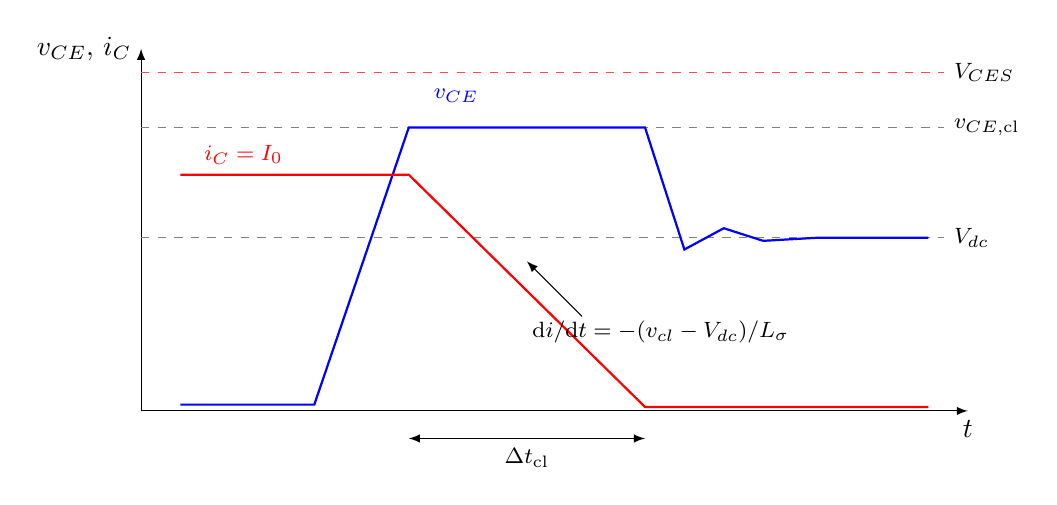
\begin{tikzpicture}[scale=1.0]
  % axes
  \draw[-latex] (0,0) -- (10.5,0) node[below]{$t$};
  \draw[-latex] (0,0) -- (0,4.6) node[left]{$v_{CE},\, i_C$};
  % reference levels
  \draw[dashed, gray] (0,2.2) -- (10.2,2.2) node[right, black]{\footnotesize $V_{dc}$};
  \draw[dashed, gray] (0,3.6) -- (10.2,3.6) node[right, black]{\footnotesize $v_{CE,\mathrm{cl}}$};
  \draw[dashed, red!70] (0,4.3) -- (10.2,4.3) node[right, black]{\footnotesize $V_{CES}$};
  % vce
  \draw[thick, blue] (0.5,0.08) -- (2.2,0.08) -- (3.4,3.6) -- (6.4,3.6)
        -- (6.9,2.05) -- (7.4,2.32) -- (7.9,2.16) -- (8.6,2.2) -- (10.0,2.2);
  \node[blue] at (4.0,4.0) {\footnotesize $v_{CE}$};
  % ic
  \draw[thick, red] (0.5,3.0) -- (3.4,3.0) -- (6.4,0.05) -- (10.0,0.05);
  \node[red] at (1.3,3.25) {\footnotesize $i_C = I_0$};
  % annotations
  \draw[latex-latex] (3.4,-0.35) -- (6.4,-0.35) node[midway, below]{\footnotesize $\Delta t_{\mathrm{cl}}$};
  \draw[-latex] (5.6,1.2) -- (4.9,1.9);
  \node at (6.6,1.0) {\footnotesize $\ud i/\ud t = -(v_{cl}-V_{dc})/L_\sigma$};
\end{tikzpicture}
\caption{Idealised clamped turn-off. The voltage rises, is caught at
$v_{CE,\mathrm{cl}}$ below the rating, and the current ramps down
linearly during $\Delta t_{\mathrm{cl}}$ while the IGBT dissipates
$E_{\mathrm{IGBT}}$.}
\label{fig:wave}
\end{figure}

\subsection{Basic versus advanced active clamping}
\label{sec:aac}

In the \emph{basic} scheme of Figure~\ref{fig:circuit} the entire
feedback current flows through the TVS stack. Its quasi-stationary value
is set by the gate network,
%
\begin{equation}
  i_{TVS} \approx
  \frac{v_{GE,\mathrm{pl}} - V_{EE}}{R_{g,\mathrm{off}}}
  \;+\; C_{ies}\frac{\ud v_{GE}}{\ud t}
  \;+\; C_{res}\frac{\ud v_{CE}}{\ud t},
  \label{eq:itvs}
\end{equation}
%
i.e.\ the current needed to hold the gate at the plateau against the
driver pull-down, plus the input-capacitance charging spike at clamp
engagement and the Miller displacement current. With the ohmic
turn-off resistors used at the 6.5\,kV level this amounts to one to a
few amperes, and the term $N r_z i_{TVS}$ in \eqref{eq:vclamp} raises
the clamp level substantially above the breakdown threshold: the
\emph{clamping factor} $v_{cl}/V_{BR,s}$ of small axial TVS devices
operated near their rated pulse current is 1.3--1.4, which, as
Section~\ref{sec:design} shows, consumes most of the margin between the
DC link and $V_{CES}$.

In \emph{advanced active clamping} (AAC), as implemented in commercial
high-voltage driver cores \cite{concept}, the TVS stack only carries a
small sense current (of the order of 0.1--0.5\,A) into a dedicated
driver input; an auxiliary stage inside the driver amplifies it,
partially or fully disabling the pull-down path (and possibly actively
sourcing gate current). The stack then operates just above its knee,
the clamping factor drops to $\approx 1.05$, and both the TVS pulse
stress and the spread of the clamp level shrink accordingly. A further
benefit is a faster loop: the response delay of the basic clamp
(TVS avalanche build-up plus gate-node charging, typically
100--200\,ns) allows a \emph{dynamic} overshoot
%
\begin{equation}
  \Delta V_{\mathrm{dyn}} \approx
  \left.\frac{\ud v_{CE}}{\ud t}\right|_{\mathrm{off}} \cdot t_{\mathrm{loop}}
  \label{eq:dyn}
\end{equation}
%
above the static clamp level; with 2--4\,kV/\textmu s typical of this
voltage class, 150\,ns of loop delay costs 300--600\,V and must be part
of the voltage budget.

\subsection{Relation to passive protections}

Active clamping does not replace the decoupling snubber: the snubber
handles the very fast local loop (module + busbar section, tens of nH)
where the clamp loop is too slow, while the clamp handles the slow,
high-energy part of the loop and abnormal events. Compared with an MOV,
the clamp level is far better defined ($\pm 5\%$ TVS tolerance versus
the soft, tolerance- and temperature-affected V--I curve of a
varistor), but the energy capability is bounded by the IGBT SOA, not by
the clamp element; an MOV bank remains the right choice when kilojoules
must be absorbed, as in the static-switch application of
Section~\ref{sec:mov}.

%=====================================================================
\section{Design for the 6.5\,kV\,/\,1000\,A Module}
\label{sec:design}
%=====================================================================

\subsection{Ratings, assumptions and protection target}

The design targets the Hitachi ABB HiPak 5SNA~1000G650300
\cite{ds5sna}: $V_{CES}=6.5$\,kV, $I_C=1000$\,A, $I_{CM}=2000$\,A, gate
limits $\pm 20$\,V, driven at $+15/-10$\,V. The following system
assumptions are used in the worked example and should be replaced by
the actual project values:

\begin{center}
\begin{tabular}{llc}
\toprule
Quantity & Symbol & Value \\
\midrule
Nominal DC link & $V_{dc}$ & 3600\,V \\
Maximum DC link (abnormal) & $V_{dc,\max}$ & 4000\,V \\
Maximum turn-off current & $I_0$ & 2000\,A \\
External commutation loop inductance & $L_\sigma$ & 300\,nH \\
Module internal inductance (order) & $L_{\mathrm{int}}$ & 10\,nH \\
Turn-off gate resistor (example) & $R_{g,\mathrm{off}}$ & 15\,$\Omega$ \\
Negative gate supply & $V_{EE}$ & $-10$\,V \\
Miller plateau at $I_0$ (estimate) & $v_{GE,\mathrm{pl}}$ & 12\,V \\
Ambient/board temperature range & --- & $-25\ldots+85\,^\circ$C \\
\bottomrule
\end{tabular}
\end{center}

The protection target is set at the module terminals:
%
\begin{equation}
  v_{CE,\max} \le V_{\mathrm{lim}} = 6.0\,\mathrm{kV},
\end{equation}
%
reserving 500\,V below $V_{CES}$ for (i) the chip-level excess
$L_{\mathrm{int}}\,|\ud i/\ud t|$ over the sensed terminal voltage,
which with \eqref{eq:didt} is only
$L_{\mathrm{int}}(v_{cl}-V_{dc})/L_\sigma \approx 60$\,V here but grows
with snappier events, and (ii) the dynamic overshoot \eqref{eq:dyn} of
the clamp loop, which is the dominant term.

\subsection{Threshold window}

The stack breakdown voltage must satisfy a two-sided inequality over
all tolerance and temperature corners:
%
\begin{align}
  N\,V_{BR,\min}\,\bigl(1+\alpha_T (T_{\min}-25\,^\circ\mathrm{C})\bigr)
     &\;\ge\; V_{dc,\max} + \Delta V_{\mathrm{rep}} ,
  \label{eq:lower}\\[2pt]
  N\,V_{BR,\max}\,\bigl(1+\alpha_T (T_{\max}-25\,^\circ\mathrm{C})\bigr)
  + N r_z i_{TVS} + v_{GE,\mathrm{pl}} + \Delta V_{\mathrm{dyn}}
     &\;\le\; V_{\mathrm{lim}} .
  \label{eq:upper}
\end{align}
%
The lower bound \eqref{eq:lower} prevents static conduction at maximum
DC link and, with the additional margin $\Delta V_{\mathrm{rep}}$,
keeps the stack out of the \emph{repetitive} turn-off overshoot so that
it is only stressed by abnormal events. Avalanche diodes above
$\sim$200\,V have a positive temperature coefficient
$\alpha_T \approx +1\cdot 10^{-3}\,/$K, so the lower corner occurs
cold and at the low tolerance limit, the upper corner hot and at the
high limit.

\subsection{TVS stack selection}

A convenient building block is the bidirectional axial transil
1.5KE440CA \cite{tvsds}: $V_{BR} = 418\ldots462$\,V at 1\,mA
($\pm5\%$), stand-off 376\,V with $\le 1$\,\textmu A leakage,
$V_C = 602$\,V at $I_{PP}=2.5$\,A (10/1000\,\textmu s), from which
$r_z \approx (602-440)/2.5 \approx 65\,\Omega$. The bidirectional
version is mandatory here: with the IGBT on, the gate ($+15$\,V) sits
above the collector ($\sim$4\,V) and a unidirectional stack would
conduct forward from gate to collector; alternatively a series blocking
diode can be added to a unidirectional stack.

\paragraph{Basic clamp, $N=10$.}
The nominal threshold is 4.40\,kV. The corners of
\eqref{eq:lower}--\eqref{eq:upper} give:

\begin{center}
\begin{tabular}{lcc}
\toprule
 & cold, low tol. & hot, high tol. \\
\midrule
$V_{BR,s}$ & $4180\times0.95 = 3.97$\,kV & $4620\times1.06=4.90$\,kV \\
$+\,N r_z i_{TVS}$ ($i_{TVS}=1.5$\,A) & --- & $+0.98$\,kV \\
$+\,v_{GE,\mathrm{pl}}$ & --- & $+0.01$\,kV \\
\midrule
result & 3.97\,kV vs.\ $V_{dc,\max}=4.0$\,kV & 5.89\,kV vs.\ $V_{\mathrm{lim}}=6.0$\,kV \\
\bottomrule
\end{tabular}
\end{center}

with $i_{TVS} \approx (12+10)/15 \approx 1.5$\,A from \eqref{eq:itvs}.
Both corners close, but with essentially no margin: the cold/low corner
sits 30\,V \emph{below} the maximum DC link (acceptable only because
near the knee the stack conducts sub-milliamp currents through
$R_{g,\mathrm{off}}$ into the low-impedance driver output, but a
standing dissipation and a slow gate lift must be checked), and the hot
side leaves nothing for the dynamic overshoot \eqref{eq:dyn}. The basic
scheme with this stack is therefore \emph{marginal}: it requires either
binned/measured TVS devices, a narrower temperature range, or a
guaranteed $i_{TVS} \lesssim 1.5$\,A.

\paragraph{Advanced clamp, $N=11$.}
With an AAC driver input (Section~\ref{sec:aac}) the sense current is
$i_{TVS}\approx0.3$\,A and one more device fits in the window:

\begin{center}
\begin{tabular}{lcc}
\toprule
 & cold, low tol. & hot, high tol. \\
\midrule
$V_{BR,s}$ & $4598\times0.95=4.37$\,kV & $5082\times1.06=5.39$\,kV \\
$+\,N r_z i_{TVS}$ ($i_{TVS}=0.3$\,A) & --- & $+0.21$\,kV \\
$+\,v_{GE,\mathrm{pl}}$ & --- & $+0.01$\,kV \\
\midrule
result & 4.37\,kV $>$ 4.0\,kV \checkmark & 5.61\,kV $\le$ 6.0\,kV \checkmark \\
\bottomrule
\end{tabular}
\end{center}

Now 370\,V of static margin remain at the bottom and $\sim$400\,V at
the top for the dynamic overshoot --- consistent with 100--150\,ns of
loop delay at 3\,kV/\textmu s. This is the recommended configuration.

\subsection{Energies and pulse stress (worked example)}

With the nominal basic-clamp level
$v_{cl} = 4400 + 975 + 12 \approx 5.4$\,kV, $I_0=2000$\,A and
$L_\sigma=300$\,nH:
%
\begin{align}
  \Delta t_{\mathrm{cl}} &= \frac{300\,\mathrm{nH}\cdot 2000\,\mathrm{A}}
        {5.4\,\mathrm{kV}-3.6\,\mathrm{kV}} \approx 0.34\,\text{\textmu s},\\
  E_{\mathrm{IGBT}} &= \tfrac12\cdot300\,\mathrm{nH}\cdot(2000\,\mathrm{A})^2
        \cdot\frac{5.4}{1.8} \approx 1.8\,\mathrm{J},\\
  E_{TVS} &\approx 5.4\,\mathrm{kV}\cdot1.5\,\mathrm{A}\cdot0.34\,\text{\textmu s}
        \approx 2.8\,\mathrm{mJ}
        \quad(\approx0.3\,\mathrm{mJ/device}),\\
  P_{TVS,\mathrm{pk}} &\approx (440+98)\,\mathrm{V}\cdot1.5\,\mathrm{A}
        \approx 0.8\,\mathrm{kW/device\ for\ }0.34\,\text{\textmu s}.
\end{align}
%
The single-event stress is trivial for a 1.5\,kW-class transil (its
short-pulse power capability is far above the 10/1000\,\textmu s
rating). The 1.8\,J absorbed by the IGBT add to the normal turn-off
energy and are acceptable as an occasional event; if the clamp engaged
at every cycle at this depth, even a few hundred hertz would add
kilowatt-level losses and violate the SOA repetition assumptions ---
hence the repetitive-overshoot margin $\Delta V_{\mathrm{rep}}$ in
\eqref{eq:lower}. Shallow grazing of the knee at the highest line
voltage is tolerable and self-limiting (the TVS TC pushes the
threshold up as the stack warms).

\subsection{Coordination with the MOV clamp (static-switch case)}
\label{sec:mov}

In the static-switch application \cite{ssprop} the turn-off of
$\sim$3\,kA against an RL load is intentionally performed against the
counter-voltage of an EPCOS B80K680 MOV bank clamping at approximately
5.5\,kV, which absorbs the multi-kilojoule load energy. An active clamp
can only coexist with the MOV if its threshold lies \emph{above} the
MOV protection level at the peak current in all corners:
%
\begin{equation}
  N\,V_{BR,\min}\,(1+\alpha_T\Delta T_{\min}) \;\ge\; V_{\mathrm{MOV}}(\hat{I})
  \approx 5.5\,\mathrm{kV}
  \;\;\Rightarrow\;\;
  N \ge \frac{5500}{418\times0.95} \approx 13.9 .
\end{equation}
%
With $N=14$ the nominal threshold is already 6.16\,kV and the clamp
level exceeds $V_{CES}$ even in the AAC variant: \emph{no feasible
window exists above a 5.5\,kV MOV}. Conversely, a threshold below the
MOV level is not admissible: during the millisecond-scale MOV
conduction the clamp would hold the IGBT in linear conduction at
$\sim$5\,kV and steer the load current (and its kilojoules) into the
silicon; Section~\ref{sec:budget} quantifies that scenario and shows it
to be fatal by more than an order of magnitude. The practical conclusions for the static switch are:
%
\begin{itemize}
  \item the MOV bank remains the sole energy clamp; the fast local
        overshoot ahead of the MOV loop is handled by the per-module
        decoupling snubber, as already foreseen;
  \item an active clamp becomes feasible only if the MOV protection
        level is lowered (more parallel columns or a lower voltage
        class) to $\lesssim 4.6$\,kV, opening an AAC window at
        $N=12$--13 --- at the cost of higher MOV standing voltage
        stress ratio;
  \item with several modules in parallel, per-module clamp networks
        with binned thresholds are required: the module with the lowest
        threshold takes the clamp energy first.
\end{itemize}

\subsection{Implementation notes}

\begin{itemize}
  \item Sense at the \emph{auxiliary} collector terminal so that the
        main-terminal inductance does not corrupt the feedback; keep
        the TVS loop short and away from the power loop.
  \item Add a small series resistor $R_s$ (a few ohms to a few tens of
        ohms) to damp the interaction between the stack capacitance and
        the gate loop; verify it does not slow the clamp response
        unacceptably.
  \item Protect the gate with a local $\pm18$\,V G--E TVS pair: during
        clamp engagement the injected spike briefly overdrives the
        gate node.
  \item The engagement spike through the stack, dominated by
        $C_{ies}$ recharge from $V_{EE}$ to the plateau, is limited
        mainly by the stack dynamic resistance and $R_s$; check the
        instantaneous TVS current against the datasheet
        $I_{PP}(t_p)$ curve.
  \item The clamp interacts with the driver's protection functions:
        desaturation detection and soft turn-off must not fight the
        clamp (a soft-turn-off ramp during clamping is generally
        beneficial; a hard re-off pulse is not).
  \item In series- or parallel-connected assemblies the clamp also
        provides dynamic voltage balancing / current derating; matched
        thresholds across positions are then essential.
\end{itemize}

%=====================================================================
\section{Thermal Limits: The Adiabatic Energy Budget}
\label{sec:adiabatic}
%=====================================================================

Equation \eqref{eq:eigbt} states how much energy the IGBT must absorb
during a clamped turn-off; it says nothing about whether it can. This
section establishes the complementary figure --- the energy the silicon
can take before an unacceptable junction temperature is reached --- and
uses it to separate the two very different situations in which an active
clamp may find itself: absorbing the commutation energy of the stray
inductance, for which it is designed, and absorbing the stored energy of
a load inductance, for which it is not.

\subsection{The adiabatic regime}

The clamped interval $\Delta t_{\mathrm{cl}}$ of \eqref{eq:didt} is
short compared with every thermal time constant of the package, so the
heat generated in the chip has no time to reach the case. All the
dissipated energy is deposited in the heat capacity of the silicon
itself, and the process is treated as \emph{adiabatic}. This is the
standard usage in the device literature \cite{lutz}, where one speaks of
the adiabatic (or short-pulse) regime of the transient thermal impedance
and of the adiabatic energy absorption capability of a device; the
qualifier belongs to the heating process, not to the energy, which is
simply the energy absorbed under adiabatic conditions.

Two consequences follow, both of which are easy to get wrong. First, the
relevant thermal capacitance is \emph{not} proportional to the mass of
the module: baseplate, solder layers and DCB substrate are thermally
decoupled from the junction on this timescale and contribute nothing.
Second, within the die itself only the fraction of the volume reached by
the heat during the pulse participates, and the dissipation over that
volume is not uniform.

The one-dimensional diffusion length in silicon,
%
\begin{equation}
  L_{\mathrm{th}} = \sqrt{\alpha\,t},
  \qquad
  \alpha_{\mathrm{Si}} = \frac{k}{\rho c}
  \approx 9\times10^{-5}\,\mathrm{m^2/s},
  \label{eq:Lth}
\end{equation}
%
with $k\approx148$\,W/(m$\cdot$K), $\rho = 2329$\,kg/m$^3$ and
$c\approx730$\,J/(kg$\cdot$K), gives the values of
Table~\ref{tab:diffusion}.

\begin{table}[htb]
\centering
\caption{Thermal diffusion length in silicon versus pulse duration.
A 6.5\,kV die is 650--700\,\textmu m thick.}
\label{tab:diffusion}
\begin{tabular}{lc}
\toprule
Pulse duration & $L_{\mathrm{th}}$ \\
\midrule
1\,\textmu s   & 10\,\textmu m \\
10\,\textmu s  & 30\,\textmu m \\
100\,\textmu s & 95\,\textmu m \\
1\,ms          & 300\,\textmu m \\
10\,ms         & 950\,\textmu m \\
\bottomrule
\end{tabular}
\end{table}

For the sub-microsecond clamp intervals of Section~\ref{sec:aac} the
heat does not even traverse the die and the package is invisible; only
above roughly 10\,ms does the baseplate begin to participate. The
adiabatic assumption is therefore safe below $\sim$100\,\textmu s and
remains a reasonable approximation into the millisecond range.

\subsection{Effective heat capacity of the die}

The whole budget follows from the volumetric heat capacity of silicon,
%
\begin{equation}
  C_v = \rho c \approx 1.7\,\mathrm{J/(cm^3 \cdot K)},
  \label{eq:Cv}
\end{equation}
%
which rises from about 1.63 at 25\,\textdegree C to 1.85\,J/(cm$^3\cdot$K)
at 150\,\textdegree C. A convenient rule of thumb is that 170\,J raise
1\,cm$^3$ of silicon by 100\,K. The adiabatic energy is then
%
\begin{equation}
  E_{\mathrm{ad}} = C_v\,V_{\mathrm{Si}}\,\Delta T_j .
  \label{eq:Ead}
\end{equation}
%
The active silicon area is not given in the datasheet \cite{ds5sna} and
must be estimated from the nominal current density, which for 6.5\,kV
chips lies in the range 35--45\,A/cm$^2$. For the 5SNA~1000G650300 this
gives an IGBT active area $A\approx25$\,cm$^2$ per switch; with a die
thickness $d = 700$\,\textmu m,
%
\begin{equation}
  V_{\mathrm{Si}} \approx 1.75\,\mathrm{cm^3}
  \quad\Longrightarrow\quad
  C_{th,\mathrm{Si}} = C_v V_{\mathrm{Si}} \approx 3.0\,\mathrm{J/K}.
  \label{eq:Cth}
\end{equation}

\subsection{Correction for non-uniform dissipation}

During clamping the device works in the active region, so the
dissipation density follows the electric field profile,
$p'''(x) = J\,E(x)$, and the local temperature rise is
$\Delta T(x) = J E(x) t/(\rho c)$. For a triangular field
$E(x) = E_{\max}(1-x/W)$ with $v_{CE,\mathrm{cl}} = E_{\max}W/2$, the
peak rise occurs at the main junction:
%
\begin{equation}
  \Delta T_{\max} = \frac{J E_{\max} t}{\rho c}
  = \frac{2 J\, v_{CE,\mathrm{cl}}\, t}{W \rho c},
  \qquad
  \frac{\Delta T_{\max}}{\Delta T_{\mathrm{unif}}} = \frac{2d}{W},
  \quad W = \frac{2 v_{CE,\mathrm{cl}}}{E_{\max}},
  \label{eq:peak}
\end{equation}
%
where $\Delta T_{\mathrm{unif}} = J v_{CE,\mathrm{cl}} t/(d\rho c)$ is
the rise obtained by spreading the same energy uniformly over the full
die thickness. With $E_{\max}\approx2\times10^5$\,V/cm and
$v_{CE,\mathrm{cl}} = 5$\,kV one obtains $W\approx500$\,\textmu m and a
peaking factor near 2.8. In a field-stop design the profile at high
voltage is closer to trapezoidal and spans almost the whole drift
region, which lowers the factor towards 1.3--1.5; under strong dynamic
avalanche the mobile carrier density reshapes it again. Equation
\eqref{eq:peak} is therefore a bounding estimate, and a factor of 2 to 3
is a reasonable engineering choice.

\subsection{Energy budget of the 5SNA~1000G650300}

Table~\ref{tab:adiabatic} applies \eqref{eq:Ead} with $C_{th,\mathrm{Si}}$
from \eqref{eq:Cth}, for a peak junction temperature limit of
120\,\textdegree C and several initial temperatures.

\begin{table}[htb]
\centering
\caption{Adiabatic energy absorption of the 5SNA~1000G650300 for a peak
junction temperature of 120\,\textdegree C, per module. The first column
assumes uniform heating of the whole die; the second includes a peaking
factor of 3.}
\label{tab:adiabatic}
\begin{tabular}{cccc}
\toprule
$T_{j,0}$ & $\Delta T_j$ & $E_{\mathrm{ad}}$ (uniform) &
$E_{\mathrm{ad}}$ (peaking $\times3$) \\
\midrule
25\,\textdegree C  & 95\,K & 285\,J & 95\,J \\
75\,\textdegree C  & 45\,K & 135\,J & 45\,J \\
100\,\textdegree C & 20\,K & 60\,J  & 20\,J \\
\bottomrule
\end{tabular}
\end{table}

The order of magnitude of the adiabatic capability is thus a few tens of
joules per module, not hundreds.

\subsection{Cross-check from the transient thermal impedance}

The chip-area estimate can be bypassed entirely by using the Foster
representation of $Z_{th(j-c)}$ from the datasheet. For
$t \ll \tau_{\min}$ the exponentials linearise, so that for an energy
$E$ delivered in a time $t$
%
\begin{equation}
  \Delta T_j = \frac{E}{t}\,Z_{th}(t)
  = \frac{E}{t}\,t\sum_i\frac{R_i}{\tau_i}
  = \frac{E}{C_{th,\mathrm{eff}}},
  \qquad
  C_{th,\mathrm{eff}} = \left(\sum_i\frac{R_i}{\tau_i}\right)^{-1} .
  \label{eq:foster}
\end{equation}
%
The whole network collapses to a single effective heat capacity,
independent of pulse duration, and for a 6.5\,kV HiPak2 it evaluates
close to the 3\,J/K of \eqref{eq:Cth}. Two caveats: datasheet Foster
fits are normally valid only above $\sim$1\,ms, and the true $Z_{th}$
follows a $\sqrt{t}$ law at short times rather than the linear law used
in \eqref{eq:foster}. Extrapolating below the shortest time constant is
therefore \emph{non-conservative} --- it underestimates the temperature
rise.

\subsection{Commutation energy versus load energy}
\label{sec:budget}

The worked example of Section~\ref{sec:aac} gives
$E_{\mathrm{IGBT}}\approx1.8$\,J for $I_0 = 2$\,kA and
$L_\sigma = 300$\,nH. Against the 45\,J available from a
75\,\textdegree C start, the margin is a factor of 25; even a
short-circuit turn-off at 6\,kA, worth some 16\,J, stays inside the
budget. In this regime the thermal limit is not the binding constraint,
and the design is governed by the repetition and SOA arguments already
made.

The picture inverts completely when the clamp is made responsible for
the energy stored in a \emph{load} inductance --- the failure mode
anticipated in Section~\ref{sec:mov}. If the device is held at
$v_{CE,\mathrm{cl}}$ for the whole decay of a current $I_0$ flowing in
an inductance $L$, then
%
\begin{equation}
  t_{\mathrm{decay}} = \frac{L I_0}{v_{CE,\mathrm{cl}} - V_{dc}},
  \qquad
  E = \tfrac12\, v_{CE,\mathrm{cl}}\, I_0\, t_{\mathrm{decay}} .
  \label{eq:Eload}
\end{equation}
%
Simulation of the static-switch case with three paralleled modules and
the clamp threshold set at (rather than above) the MOV protection level
gives, per module, $I_0 = 850$\,A, $v_{CE,\mathrm{cl}} = 5.5$\,kV and
$t_{\mathrm{decay}} = 1.5$\,ms, hence
%
\begin{equation}
  E = \tfrac12\cdot5.5\,\mathrm{kV}\cdot850\,\mathrm{A}\cdot1.5\,\mathrm{ms}
  \approx 3.5\,\mathrm{kJ},
  \qquad
  \Delta T_j = \frac{3.5\,\mathrm{kJ}}{3.0\,\mathrm{J/K}}
  \approx 1170\,\mathrm{K},
\end{equation}
%
where the second figure already uses the most favourable assumption
available: the entire die volume, heated uniformly, with no peaking
factor. It still exceeds the melting point of silicon
(1414\,\textdegree C). The average dissipated power, 2.3\,MW, is more
than two orders of magnitude above what the die can conduct away in
1.5\,ms; destruction is certain and occurs within the first tens of
microseconds of the event.

The conclusion is structural rather than numerical. An active clamp is a
\emph{voltage-limiting} function, not an \emph{energy-absorbing} one.
Adding paralleled modules does not repair the situation --- more than a
hundred would be needed to bring the per-module energy inside
Table~\ref{tab:adiabatic} --- and the sharing between them in the active
region is the worst possible. Magnetic energy stored in a load
inductance must be taken by an element designed for it (MOV bank, dump
resistor with crowbar, or a freewheeling path), and the semiconductor
clamp threshold must be coordinated \emph{above} the protection level of
that element, so that the device turns fully off. Where the two levels
coincide, the device operating in the active region is always the softer
path and takes the whole energy: this is precisely why
Section~\ref{sec:mov} concludes that no admissible window exists above a
5.5\,kV MOV.

\subsection{Limits other than junction temperature}
\label{sec:otherlimits}

The temperature criterion above is a volume average, necessary but not
sufficient. Several mechanisms act locally and can destroy the device
well below the computed energy:

\begin{itemize}
  \item \textbf{Current filamentation.} The gate sits close to
        threshold, where the transconductance has a strong negative
        temperature coefficient; the current does not stay uniformly
        distributed over cells and chips, and a filament carrying
        several times the average density invalidates the
        volume-averaged estimate.
  \item \textbf{Dynamic avalanche.} The mobile carrier density adds to
        the ionised doping charge in the space-charge region, raising
        the peak field and displacing it towards the field-stop layer
        \cite{lutz}.
  \item \textbf{Leakage-driven thermal runaway and latch-up}, which set
        in well below the intrinsic temperature of silicon.
  \item \textbf{Sharing between paralleled modules.} Active clamping is
        the worst sharing condition: threshold spread translates
        directly into current unbalance, and the module clamping first
        takes a disproportionate share --- hence the binned-threshold
        requirement of Section~\ref{sec:mov}.
\end{itemize}

The adiabatic budget is therefore best used as a screening criterion. It
tells whether a design is far from the thermal limit, which is the case
for stray-inductance clamping and emphatically not the case for load
energy absorption; the manufacturer's RBSOA and clamping specifications
remain the binding constraint.

%=====================================================================
\section{Simscape Model \texttt{tvs\_clamp}}
%=====================================================================

\subsection{Scope and equations}

The component \texttt{tvs\_clamp} (Appendix~\ref{app:code}) models the
complete stack --- $N$ series devices per string, $M$ parallel strings
--- as a single electrical two-terminal, intended to be wired from the
collector (auxiliary terminal) to the gate node of \texttt{igbt\_dyn}
in a double-pulse or application-level simulation. It follows the same
conventions as the other components of the personal \texttt{.ssc}
library.

The constitutive relation is a symmetric, purely algebraic
piecewise-linear characteristic with a smoothed knee, in parallel with
leakage and a lumped junction capacitance:
%
\begin{align}
  i &= \frac{v}{R_{\mathrm{ls}}}
     + \frac{\mathrm{sp}(v - V_{\mathrm{brs}}) - \mathrm{sp}(-v - V_{\mathrm{brs}})}{r_{\mathrm{zs}}}
     + C_s \frac{\ud v}{\ud t},
  \label{eq:model}\\[4pt]
  \mathrm{sp}(x) &= \tfrac12\left(x + \sqrt{x^2 + \Delta V_s^2}\,\right),
  \label{eq:softplus}
\end{align}
%
with the stack equivalents
%
\begin{equation}
  V_{\mathrm{brs}} = N V_{BR}\bigl(1+\alpha_T(T_{\mathrm{dev}}-T_{\mathrm{ref}})\bigr),
  \quad
  r_{\mathrm{zs}} = \frac{N r_z}{M},
  \quad
  R_{\mathrm{ls}} = \frac{N R_{\mathrm{leak}}}{M},
  \quad
  C_s = \frac{M C_j}{N},
  \quad
  \Delta V_s = N\,\Delta V .
\end{equation}
%
The function $\mathrm{sp}(x)$ is a softplus-like smooth positive part:
it equals $\max(0,x)$ away from the knee and rounds it over a width of
order $\Delta V_s$. Being algebraic (no exponentials), it cannot
overflow and behaves well with stiff solvers --- the same reasoning
used in the depletion clamps of \texttt{diode\_rr}. The two mirrored
terms in \eqref{eq:model} make the characteristic odd, i.e.\ the stack
is bidirectional, matching the CA-suffix devices; for a unidirectional
stack with series blocking diode, the negative branch can be removed
and a forward-diode branch added.

\subsection{Parameters and defaults}

Defaults describe the 1.5KE440CA:

\begin{center}
\begin{tabular}{llll}
\toprule
Parameter & Symbol & Default & Source / note \\
\midrule
\texttt{N} & $N$ & 10 & series devices per string \\
\texttt{M} & $M$ & 1 & parallel strings \\
\texttt{Vbr} & $V_{BR}$ & 440\,V & $\pm5\%$ @ 1\,mA \cite{tvsds} \\
\texttt{rz} & $r_z$ & 65\,$\Omega$ & $(V_C-V_{BR})/I_{PP}=(602-440)/2.5$ \\
\texttt{Rleak} & $R_{\mathrm{leak}}$ & 400\,M$\Omega$ & 376\,V / $\le1$\,\textmu A \\
\texttt{Cj} & $C_j$ & 100\,pF & order of magnitude; take from datasheet \\
\texttt{dV} & $\Delta V$ & 8\,V & knee smoothing per device \\
\texttt{alphaT} & $\alpha_T$ & $1\cdot10^{-3}$\,/K & avalanche TC, $V_{BR}>200$\,V \\
\texttt{Tdev}, \texttt{Tref} & $T_{\mathrm{dev}}, T_{\mathrm{ref}}$ & 25\,$^\circ$C & fixed device temperature \\
\bottomrule
\end{tabular}
\end{center}

Tolerance corners are explored by scaling \texttt{Vbr} to
418/462\,V and sweeping \texttt{Tdev}; there is deliberately no Monte
Carlo machinery inside the component.

\subsection{Limitations}

(i) No self-heating: $V_{BR}$ shifts during a long clamp pulse are not
reproduced (conservative for the upper corner if $T_{\mathrm{dev}}$ is
set hot). (ii) $r_z$ is constant, while real transils are sublinear at
high pulse current; near and above $I_{PP}$ the model overestimates the
clamp voltage --- acceptable, since the design intent is precisely to
keep $i_{TVS}$ small. (iii) The avalanche build-up delay (ns range) is
neglected; the dominant loop delay comes from the gate node and must be
represented by the driver/gate model, not by the TVS.

\subsection{Suggested validation}

Reuse the double-pulse bench built around \texttt{igbt\_dyn} with the
5SNA~1000G650300 parameter set: connect \texttt{tvs\_clamp} from the
collector node to the gate node behind $R_{g,\mathrm{off}}$, drive with
the ideal $+15/-10$\,V source, and sweep $I_0$ (500--2000\,A) and
$L_\sigma$ (100--600\,nH). Check: (a) the $v_{CE}$ plateau against
\eqref{eq:vclamp}, (b) $\Delta t_{\mathrm{cl}}$ and the current slope
against \eqref{eq:didt}, (c) $i_{TVS}$ against \eqref{eq:itvs}
including the engagement spike, (d) energies via integrated
$v\!\cdot\!i$ against \eqref{eq:eigbt}--\eqref{eq:etvs}. If the solver
struggles at the knee, increase \texttt{dV} (the clamp level error is
of order $\Delta V_s/2$ at most) before touching tolerances, as done
for the tail-charge equations of \texttt{igbt\_dyn}.

%=====================================================================
\section{Conclusion}
%=====================================================================

Active clamping turns the 6.5\,kV IGBT itself into its own overvoltage
absorber at the cost of a signal-level TVS network. For the
5SNA~1000G650300 on a 3.6\,kV link, a stack of ten 1.5KE440CA devices
closes the design window only marginally in the basic scheme, while
eleven devices with an advanced (driver-assisted) clamp input leave
healthy static and dynamic margins; in the MOV-clamped static switch no
admissible window exists above the 5.5\,kV varistor level, and the MOV
must remain the sole energy clamp. The adiabatic budget of
Section~\ref{sec:adiabatic} explains why the coordination is not
negotiable: the die can absorb a few tens of joules before reaching
120\,\textdegree C, so the sub-joule commutation energy is comfortably
within reach while the kilojoules of a load inductance are not, by a
factor of forty. The \texttt{tvs\_clamp} Simscape
component captures the stack with a numerically robust smoothed
breakdown characteristic and slots directly into the existing
\texttt{igbt\_dyn} double-pulse bench for time-domain verification of
clamp level, timing and energies.

%=====================================================================
\begin{thebibliography}{9}

\bibitem{volke} A. Volke and M. Hornkamp, \emph{IGBT Modules ---
Technologies, Driver and Application}, 2nd ed., Infineon Technologies,
Munich, 2012.

\bibitem{lutz} J. Lutz, H. Schlangenotto, U. Scheuermann, and
R. De Doncker, \emph{Semiconductor Power Devices --- Physics,
Characteristics, Reliability}, 2nd ed., Springer, 2018.

\bibitem{abb2053} ABB Switzerland Ltd, Semiconductors, ``Applying
IGBTs,'' Application Note 5SYA 2053.

\bibitem{concept} CT-Concept Technologie AG / Power Integrations,
application literature on the Advanced Active Clamping function of
SCALE gate-driver cores for high-voltage IGBTs.

\bibitem{ds5sna} Hitachi ABB Power Grids, ``5SNA 1000G650300 HiPak IGBT
Module,'' Data Sheet 5SYA 1465.

\bibitem{tvsds} STMicroelectronics / Vishay, ``1.5KE series ---
1500\,W Transil / TVS diodes,'' data sheet.

\bibitem{snubdes} D. Bagnara, \emph{Snubber Design Guidelines for a
High-Current IGBT Half-Bridge Leg}, internal note.

\bibitem{snubpar} D. Bagnara, \emph{Snubbers for Paralleled 5SNA
1000G650300 IGBT Modules}, internal note.

\bibitem{movnote} D. Bagnara, \emph{The EPCOS SIOV-B80K680 Block
Varistor: Characteristics and Application Sizing}, internal note.

\bibitem{ssprop} D. Bagnara, \emph{High-Current Static Switch ---
Preliminary Proposal}, internal note.

\end{thebibliography}

%=====================================================================
\appendix
\section{Source of \texttt{tvs\_clamp.ssc}}
\label{app:code}
%=====================================================================

\lstset{language=Matlab, morekeywords={component,nodes,parameters,
variables,branches,intermediates,equations,end,Access,private}}
\begin{lstlisting}
component tvs_clamp
% TVS Clamp Stack
% Bidirectional TVS (transil) stack for IGBT active clamping studies:
% N series devices per string, M parallel strings, modelled as a single
% two-terminal element. Symmetric avalanche breakdown with a smooth,
% purely algebraic knee (no exponentials), constant dynamic resistance,
% sub-breakdown leakage and a lumped junction capacitance. The breakdown
% voltage has a linear temperature coefficient; the device temperature is
% a fixed parameter (no self-heating).
%
% Default parameters: 1.5KE440CA (V_BR = 440 V +/-5% @ 1 mA,
% V_C = 602 V @ I_PP = 2.5 A -> r_z ~ 65 Ohm, V_RM = 376 V / I_R <= 1 uA
% -> R_leak ~ 400 MOhm). Intended use: collector-to-gate clamp network
% together with igbt_dyn (e.g. 5SNA 1000G650300 parameter set).

  nodes
    p = foundation.electrical.electrical; % +:left
    n = foundation.electrical.electrical; % -:right
  end

  parameters
    N     = {10,     '1'   }; % Series devices per string, N
    M     = {1,      '1'   }; % Parallel strings, M
    Vbr   = {440,    'V'   }; % Breakdown voltage per device @ Tref, V_BR
    rz    = {65,     'Ohm' }; % Dynamic resistance per device, r_z
    Rleak = {400e6,  'Ohm' }; % Sub-breakdown leakage resistance per device
    Cj    = {100e-12,'F'   }; % Junction capacitance per device, C_j
    dV    = {8,      'V'   }; % Knee smoothing voltage per device
    alphaT= {1e-3,   '1/K' }; % Breakdown temperature coefficient, alpha_T
    Tdev  = {298.15, 'K'   }; % Device temperature
    Tref  = {298.15, 'K'   }; % Reference temperature for V_BR
  end

  parameters (Access = private)
    Vbrs = N*Vbr;      % nominal stack breakdown (before TC correction)
    rzs  = N*rz/M;     % stack dynamic resistance
    Rls  = N*Rleak/M;  % stack leakage resistance
    Cs   = M*Cj/N;     % stack capacitance
    dVs  = N*dV;       % stack knee smoothing voltage
  end

  variables
    v = {0, 'V'}; % Voltage
    i = {0, 'A'}; % Current
  end

  branches
    i : p.i -> n.i;
  end

  intermediates
    % Temperature-corrected stack breakdown voltage
    VbrT = Vbrs*(1 + alphaT*(Tdev - Tref));
    % Smooth positive-part (softplus-like, algebraic: max(0,x) with
    % rounding over ~dVs around the knee, safe for stiff solvers)
    xp  = v - VbrT;
    xn  = -v - VbrT;
    spp = 0.5*(xp + sqrt(xp^2 + dVs^2));
    spn = 0.5*(xn + sqrt(xn^2 + dVs^2));
  end

  equations
    v == p.v - n.v;
    i == v/Rls + (spp - spn)/rzs + Cs*der(v);
  end

end
\end{lstlisting}

\end{document}
